\documentclass[tikz,border=2pt]{standalone}
% Preámbulo común de los diagramas TikZ (misma paleta y letra que las notas)
\usepackage[T1]{fontenc}\usepackage[utf8]{inputenc}
\usepackage{libertinus}\usepackage{libertinust1math}
\usepackage[defaultsans,scale=0.92]{lato}
\usepackage{amsmath,amssymb,bm}
\usepackage{tikz}\usetikzlibrary{calc,positioning,arrows.meta,shapes.geometric,decorations.pathreplacing,decorations.pathmorphing,fit,backgrounds}
\definecolor{snlazul}{HTML}{1E5AA8}\definecolor{snlnoche}{HTML}{14213D}\definecolor{snlvioleta}{HTML}{6C4AB6}
\definecolor{snlcoral}{HTML}{D1495B}\definecolor{snlambar}{HTML}{E09F3E}\definecolor{snlverde}{HTML}{2A9D8F}
\definecolor{snlteal}{HTML}{0F7173}\definecolor{snlgris}{HTML}{5C677D}\definecolor{snlfondo}{HTML}{F4F6FA}
\tikzset{>={Stealth[length=2.2mm]},
  bloque/.style={draw=#1,fill=#1!8,thick,rounded corners=2pt,minimum height=11mm,minimum width=20mm,align=center,font=\small},
  bloque/.default=snlazul,
  suma/.style={draw=snlnoche,thick,circle,inner sep=0pt,minimum size=5mm},
  flecha/.style={->,thick,draw=snlnoche},
  etq/.style={font=\small,text=snlnoche},
  nota/.style={font=\footnotesize\sffamily,text=snlgris,align=center}}

\begin{document}
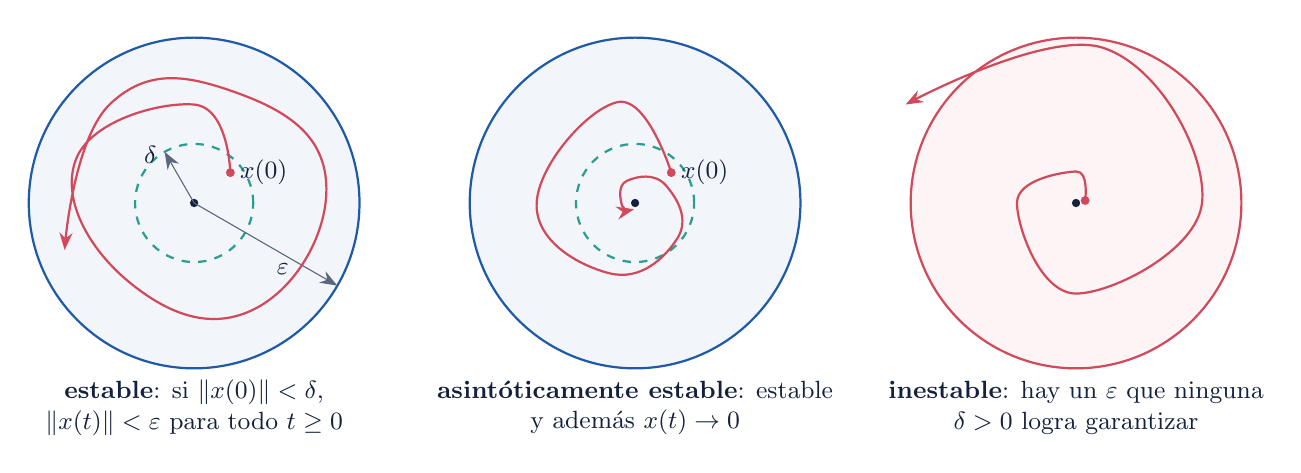
\begin{tikzpicture}
 \begin{scope}
  \fill[snlazul!6] (0,0) circle (2.1);
  \draw[snlazul,thick] (0,0) circle (2.1);
  \draw[snlverde,thick,dashed] (0,0) circle (0.75);
  \fill[snlnoche] (0,0) circle (1.5pt);
  \draw[snlgris,->] (0,0) -- (-30:2.1) node[pos=0.62,below,etq]{$\varepsilon$};
  \draw[snlgris,->] (0,0) -- (120:0.75) node[pos=0.95,left,etq]{$\delta$};
  \fill[snlcoral] (40:0.6) circle (1.6pt) node[right,etq]{$x(0)$};
  \draw[snlcoral,thick,->] plot[smooth,tension=0.8] coordinates {(40:0.6) (90:1.25) (160:1.6) (230:1.3) (300:1.55) (10:1.7) (70:1.5) (130:1.65) (200:1.75)};
  \node[etq,align=center] at (0,-2.6) {\textbf{estable}: si $\|x(0)\|<\delta$,\\ $\|x(t)\|<\varepsilon$ para todo $t\ge0$};
 \end{scope}
 \begin{scope}[xshift=5.6cm]
  \fill[snlazul!6] (0,0) circle (2.1);
  \draw[snlazul,thick] (0,0) circle (2.1);
  \draw[snlverde,thick,dashed] (0,0) circle (0.75);
  \fill[snlnoche] (0,0) circle (1.5pt);
  \fill[snlcoral] (40:0.6) circle (1.6pt) node[right,etq]{$x(0)$};
  \draw[snlcoral,thick,->] plot[smooth,tension=0.8] coordinates {(40:0.6) (100:1.3) (180:1.25) (250:0.95) (320:0.7) (30:0.45) (110:0.3) (190:0.17) (260:0.08)};
  \node[etq,align=center] at (0,-2.6) {\textbf{asintóticamente estable}: estable\\ y además $x(t)\to0$};
 \end{scope}
 \begin{scope}[xshift=11.2cm]
  \fill[snlcoral!6] (0,0) circle (2.1);
  \draw[snlcoral,thick] (0,0) circle (2.1);
  \fill[snlnoche] (0,0) circle (1.5pt);
  \fill[snlcoral] (15:0.12) circle (1.6pt);
  \draw[snlcoral,thick,->] plot[smooth,tension=0.7] coordinates {(15:0.12) (90:0.4) (180:0.75) (270:1.15) (0:1.6) (80:2.0) (150:2.5)};
  \node[etq,align=center] at (0,-2.6) {\textbf{inestable}: hay un $\varepsilon$ que ninguna\\ $\delta>0$ logra garantizar};
 \end{scope}
\end{tikzpicture}
\end{document}
